\documentclass[14pt, xcolor=svgnames]{beamer}

\usepackage[dvipsnames]{xcolor}
\usepackage{tikz}
\usetikzlibrary{angles,quotes}
% Definition of a square!
\def\Square at (#1, #2) length (#3) #4; {
    \node at (#1, #2) {\small #4};
    \draw (#1 - #3, #2 - #3) rectangle (#1 + #3,#2 + #3);
}

\usetheme{Warsaw}
\usecolortheme{orchid}

\setbeamertemplate{navigation symbols}{}
\setbeamertemplate{headline}{}
\expandafter\def\expandafter\insertshorttitle\expandafter{%
  \insertshorttitle\hfill%
  \insertframenumber\,/\,\inserttotalframenumber}
\setbeamercovered{transparent}

\newcommand{\Green}[1]{\textcolor{Green}{#1}}
\newcommand{\Purple}[1]{\textcolor{Purple}{#1}}
\newcommand{\Blue}[1]{\textcolor{blue}{#1}}

\title{Operad Structure of 4D Braids}
\author[Nicholas Bertollo]{Nicholas Bertollo \\[1cm]  {\small Dr. Zsuzsanna Dancso}}
\institute{University of Sydney}
\date[University of Sydney]{\today}

\begin{document}

\maketitle

\begin{frame}{Itinerary}
\tableofcontents
\end{frame}

\section{What are Structures?}

\begin{frame}{Structures}
    Consider the integers under addition:
    \begin{gather*}
        \cdots -5, -4, -3, -2, -1, 0, 1, 2, 3, 4, 5 \cdots
    \end{gather*}
    And question what \Blue{properties} they have? \vspace{1cm}
    
    We can name many properties, however here are some. 
\end{frame}

\begin{frame}
    Consider the integers \( a \), \( b \), and \( c \). 
    \begin{enumerate}
        \item \( a + b \) is an integer \hfill (Closure)
        \item \( ( a + b ) + c = a + ( b + c ) \) \hfill (Associative)
        \item \( a + 0 = a \) \hfill (Identity)
        \item \( a + (-a) = 0 \) \hfill (Inverses)
    \end{enumerate}
    \begin{center}
        \fbox{Objects with these properties are called \Green{Groups}.}
    \end{center} \vspace{0.2cm}
    A \Green{Group} is a type of \Blue{structure}. \vfill
    \setbeamercovered{invisible}
    \pause
    \begin{center}
        But... why do we care?
    \end{center} \vfill
\end{frame}

\begin{frame}
    Consider Rotations in 2D under the operation of composition, e.g. \\
    \begin{center}
    % \hfill
    % \( \delta_\alpha = \) 
    \begin{tikzpicture}
        \coordinate (o) at (0,0);
        \coordinate (r) at (30:1);
        \coordinate (x) at (1.2,0);
        \coordinate (l) at (-1.2, 0);
        \draw[->] (-1,0) -- (1.2,0) node[right] {$x$}; 
        \draw[->] (0,-1) -- (0,1.2) node[above] {$y$};
        \draw[->] (o) -- (r) node[right] {}; 
        \pic[draw, "$\alpha$", angle eccentricity=1.5] {angle = x--o--r};
        \node[left] at (l) {\( \delta_\alpha = \) };
    \end{tikzpicture}
    \hspace{1cm}
    % \( \delta_\beta = \) 
    \begin{tikzpicture}
        \coordinate (o) at (0,0);
        \coordinate (r) at (120:1);
        \coordinate (x) at (1.2,0);
        \coordinate (l) at (-1.2, 0);
        \draw[->] (-1,0) -- (1.2,0) node[right] {$x$}; 
        \draw[->] (0,-1) -- (0,1.2) node[above] {$y$};
        \draw[->] (o) -- (r) node[right] {}; 
        \pic[draw, "$\beta$", angle eccentricity=1.5] {angle = x--o--r};
        \node[left] at (l) {\( \delta_\beta = \) };
    \end{tikzpicture}
    \hfill
    \end{center}
    \pause
    Composing gets us:
    \begin{center}
    % \( \delta_\alpha \circ \delta_\beta = \) 
    \begin{tikzpicture}
        \coordinate (o) at (0,0);
        \coordinate (lineB) at (150:1);
        \coordinate (lineA) at (30:1);
        \coordinate (x) at (1.2,0);
        \coordinate (l) at (-1.2, 0);
        \coordinate (r) at (1.2, 0);
        \draw[->] (-1,0) -- (1.2,0) node[right] {}; 
        \draw[->] (0,-1) -- (0,1.2) node[above] {};
        \draw[->] (o) -- (lineA) node[right] {}; 
        \draw[->] (o) -- (lineB) node[right] {}; 
        \pic[draw, "$\alpha$", angle eccentricity=1.5] {angle = x--o--lineA};
        \pic[draw, "$\beta$", angle eccentricity=1.5, left] {angle = lineA--o--lineB};
        \node[left] at (l) {\( \delta_\alpha \circ \delta_\beta = \)};
        \node[right] at (r) {\( = \delta_{\alpha + \beta}\)};
    \end{tikzpicture}
    \hfill
    \end{center}
\end{frame}

\begin{frame}
    Let's think about the \Blue{structure} of rotations. 
    Consider the rotations \( \delta_\alpha \), \( \delta_\beta \), and \( \delta_\gamma \). 
    \begin{enumerate}
        \item \( \delta_\alpha \circ \delta_\beta \) is an rotation \hfill (Closure)
        \item \( ( \delta_\alpha \circ \delta_\beta ) \circ \delta_\gamma = \delta_\alpha \circ ( \delta_\beta \circ \delta_\gamma ) \) \hfill (Associative)
        \item \( \delta_\alpha \circ \delta_0 = \delta_\alpha \) \hfill (Identity)
        \item \( \delta_\alpha \circ (\delta_{-\alpha}) = \delta_0 \) \hfill (Inverses)
    \end{enumerate} 
    The exact same as before!
    \vfill
    \pause
    \begin{center}
        \fbox{Rotations in 2D form a \Green{Group}!}
    \end{center}
\end{frame}

\begin{frame}
    \begin{block}{Point}
        We do not have to study situations, we can instead study the \Blue{structure} of the situation. 
    \end{block}
    
    \begin{block}{Definition}
        A \Blue{structure} is a \Blue{set of objects} with some \Blue{rules} defined on them.  
    \end{block} \vfill
    \begin{center}
        \framebox{
            An \Purple{Operad} is a type of \Blue{structure}. 
        }
    \end{center}
\end{frame}

\section{What are Operads?}

\begin{frame}{Operads}
    \Purple{Operads} are best learnt by example. \\
    Consider some named squares located inside a square. \\
    \begin{center}
        \begin{tikzpicture}
            \node[left] at (-1.5, 0) {\( A = \)};
            \Square at (0, 0) length (1.5) {}; % Main square
            \Square at (-0.8, 0.6) length (0.5) {\( A_1 \)};
            \Square at (0.5, 0.7) length (0.75) {\( A_2 \)};
            \Square at (0.2, -0.8) length (0.6) {\( A_3 \)};
        \end{tikzpicture} \hspace{1cm}
        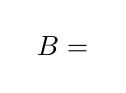
\begin{tikzpicture}
            \node[left] at (-1.5, 0) {\( B = \)};
            \Square at (0, 0) length (1.5) {};
            \Square at (-0.6, -0.6) length (0.5) {\( B_1 \)};
            \Square at (0.4, 0.7) length (0.7) {\( B_2 \)};
        \end{tikzpicture} 
        \hfill
    \end{center} 
    What happens when you compose \( B \) within \( A_2 \)?
\end{frame}

\begin{frame}
    We denote composition into the second spot as \( \circ_2 \), let's perform \( A \circ_2 B \). \\
    {
    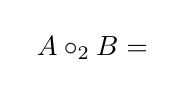
\begin{tikzpicture}
        \node[left] at (-1.5, 0) {\( A \circ_2 B= \)};
        \Square at (0, 0) length (1.5) {}; % Main square
        \Square at (-0.8, 0.6) length (0.5) {\( A_1 \)};
        \Square at (0.5, 0.7) length (0.75) {\( A_2 \)};
        \Square at (0.2, -0.8) length (0.6) {\( A_3 \)};
    \end{tikzpicture} 
    \begin{tikzpicture}
        \node[left] at (-1.5, 0) {\( \circ_2 \)};
        \Square at (0, 0) length (1.5) {};
        \Square at (-0.6, -0.6) length (0.5) {\( B_1 \)};
        \Square at (0.4, 0.7) length (0.7) {\( B_2 \)};
    \end{tikzpicture} \hfill\\
    \begin{tikzpicture}
        \node[left] at (-1.5, 0) {\( A \circ_2 B= \)};
        \Square at (0, 0) length (1.5) {}; 
        \Square at (-0.8, 0.6) length (0.5) {\( A_1 \)};
        % \Square at (0.5, 0.7) length (0.75) {};
        \draw[densely dashed] (-0.25, -0.05) rectangle (1.25, 1.45);
        \Square at (0.5 - 0.3, 0.7 - 0.3) length (0.25) {\( B_1 \)};
        \Square at (0.5 + 0.2, 0.7 + 0.35) length (0.35) {\( B_2 \)};
        \Square at (0.2, -0.8) length (0.6) {\( A_3 \)};
    \end{tikzpicture} \hfill \\
    }
    The dotted line is not apart of \( A \circ_2 B \), it is there purely for explanatory reasons.  
\end{frame}

\begin{frame}
    \begin{block}{Point}
        An \Purple{Operad} generalises composition for multi-dimensional objects. 
    \end{block}
    \begin{block}{Definition}
        We call a function \( n \)-ary if it has \( n \) inputs and \( 1 \) output. 
    \end{block}
    Let's define: \\
    \begin{center}
        A \( 3 \)-ary function, \( A(x_1, x_2, x_3) \) \\ 
        And a \( 2 \)-ary function, \( B(y_1, y_2) \)
    \end{center}
\end{frame}

\begin{frame}
    \( A \circ_2 B \) is a \( 4 \)-ary function such that:
    \[ A \circ_2 B(x_1, y_1, y_2, x_3) = A(x_1, \underbrace{B(y_1, y_2)}_{\text{Replaces }x_2}, x_3) \]
    This forms an \Purple{Operad}\footnote{Conditions/Rigour Applies.}.
    \vfill
    \begin{block}{Question}
    Can you see the parallel between this and the squares?
    \end{block}
    \vfill
\end{frame}
    
\section{3D Braids!}
\begin{frame}{3D Braids}
    Think of 3D braids as a movie, where time is our third dimension. 
    \begin{center}
    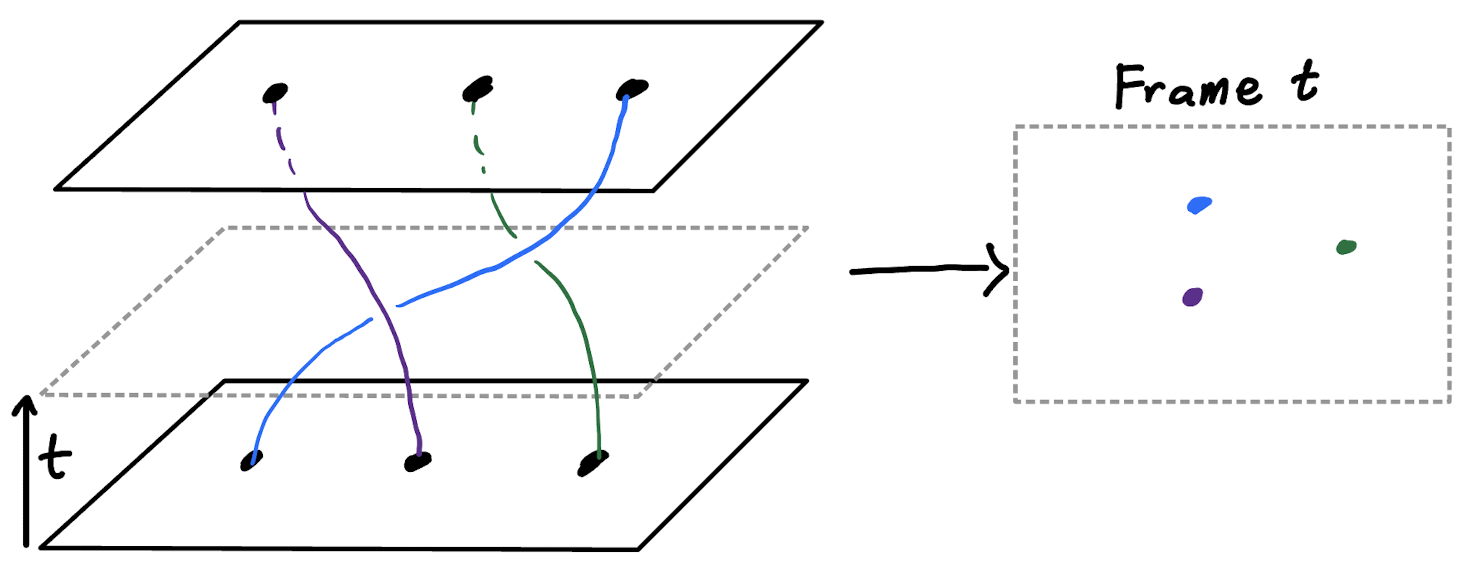
\includegraphics[scale = 0.2]{images/movie representation of a braid.png}
    \end{center}
    % Input picture of 3D braid and a single frame. 

    At time \( t \), we have a snapshot of what the braid looks like.  
\end{frame}

\begin{frame}
    \begin{center}
        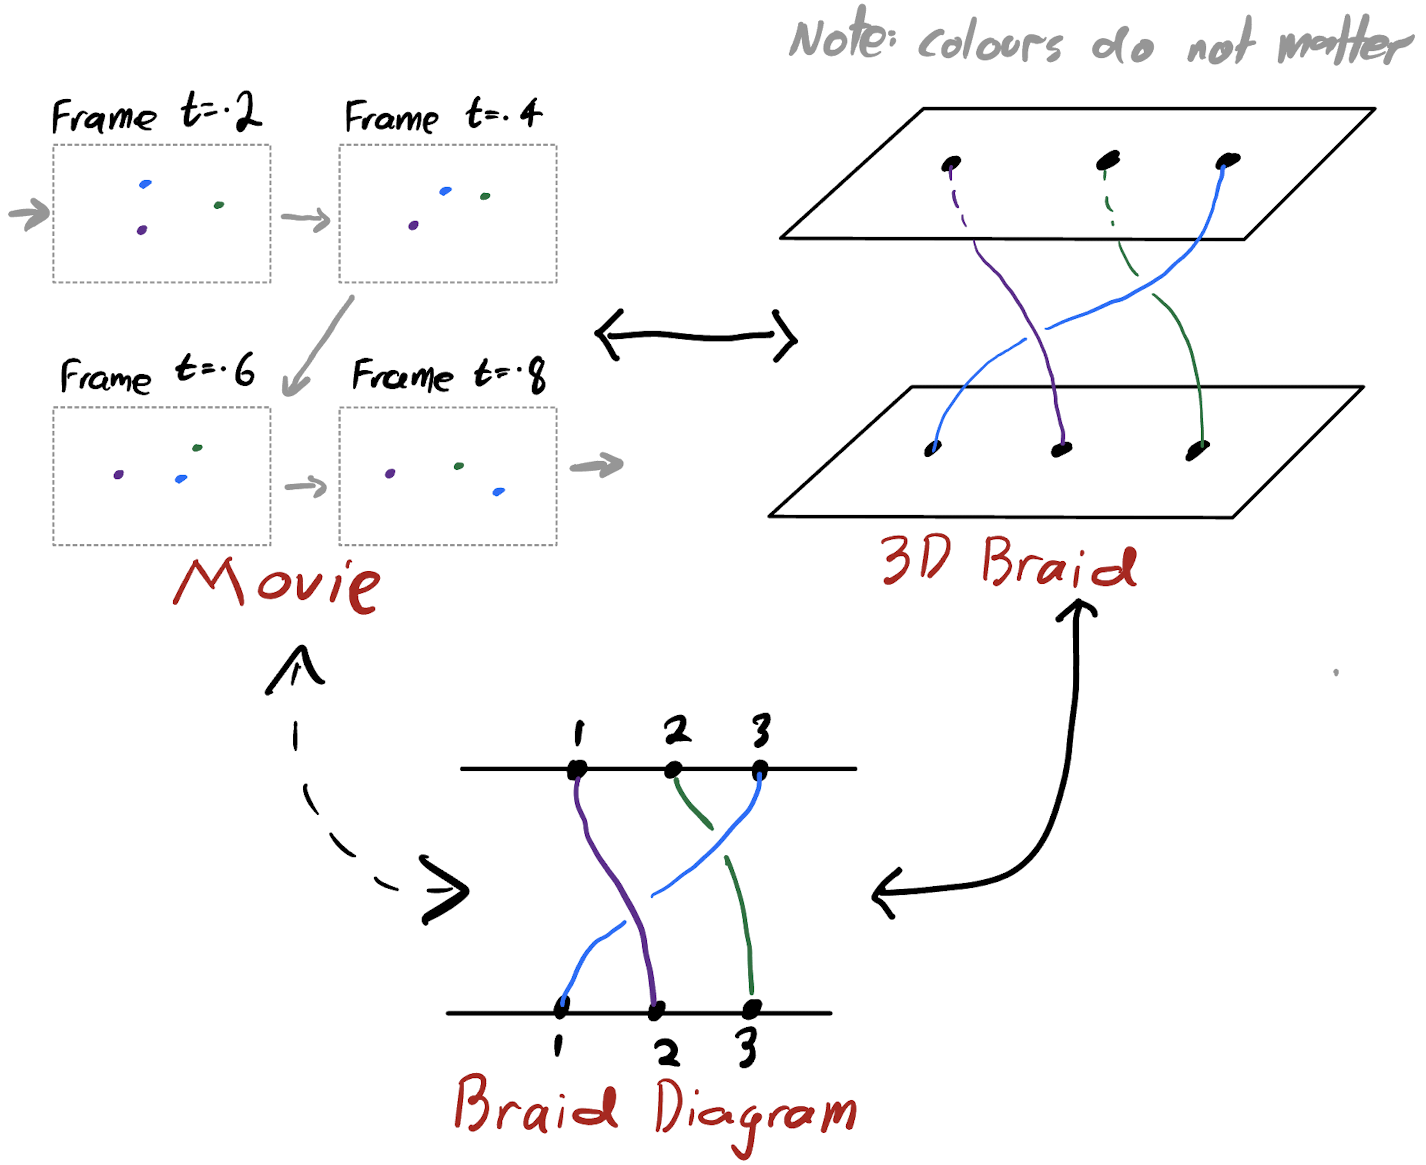
\includegraphics[scale = 0.2]{images/representations of braids.png}
    \end{center}
    % This contains a picture of how a braid can be thought of as a movie, a braid, and a braid diagram. 
\end{frame}

\section{The 3D Canonical Braid Operad}

\begin{frame}{The Canonical 3D Braid Operad}
    But we want to compose braids! \\
    Let's define composition as replacement, for example:

    \begin{center}
        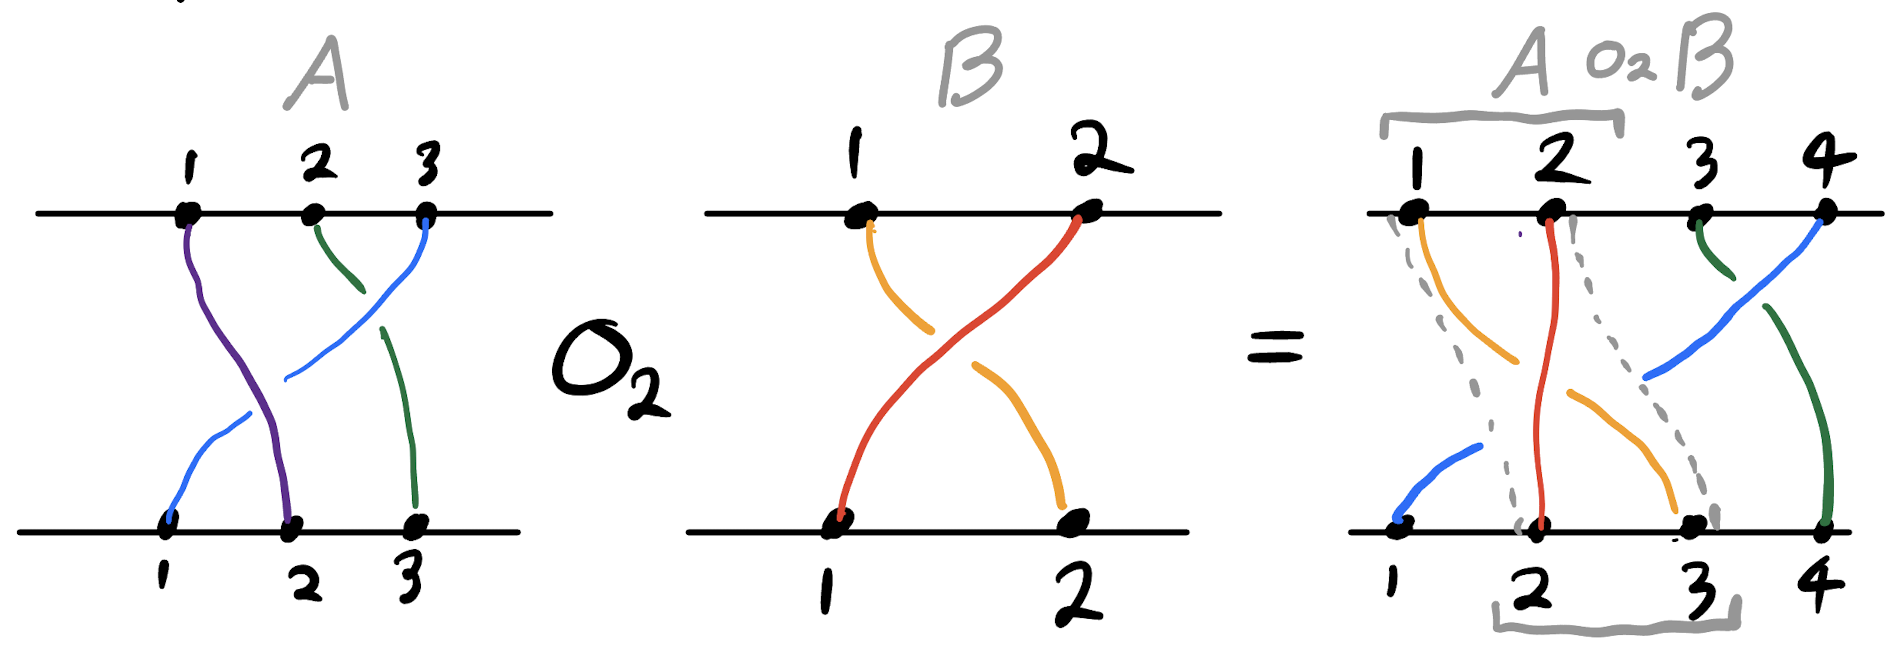
\includegraphics[scale = 0.16]{images/composition in the usual braid operad.png}
    \end{center}
    You can see we're replacing the second strand of \( A \) with the braid \( B \). 
    % Picture of that shows replacing a strand with a braid. 
    
\end{frame}

\begin{frame}
    It is known that \( 3 \)D braids form an \Purple{Operad} \textcolor{Red}{Canonically}. 
    This means that there is only a single reasonable choice for how composition might be defined for braids in \( 3 \)D. 
    Does this work for \( 4 \)D braids however?
\end{frame}

\section{4D Braids!}
\begin{frame}{\( 4 \)D braids}
    You cannot braid \( 1 \)D things in \( 4 \)D! \\
    As lines can ``pass into the \( 4 \)th dimension'' and go around each other. \\
    \onslide<2->{\textcolor{Red}{All \( 4 \)D braids of \( 1 \)D strands are uninteresting.}}
\end{frame}

\begin{frame}
    Therefore, we are infact braiding tubes in \( 4 \)D.
    \begin{center}
        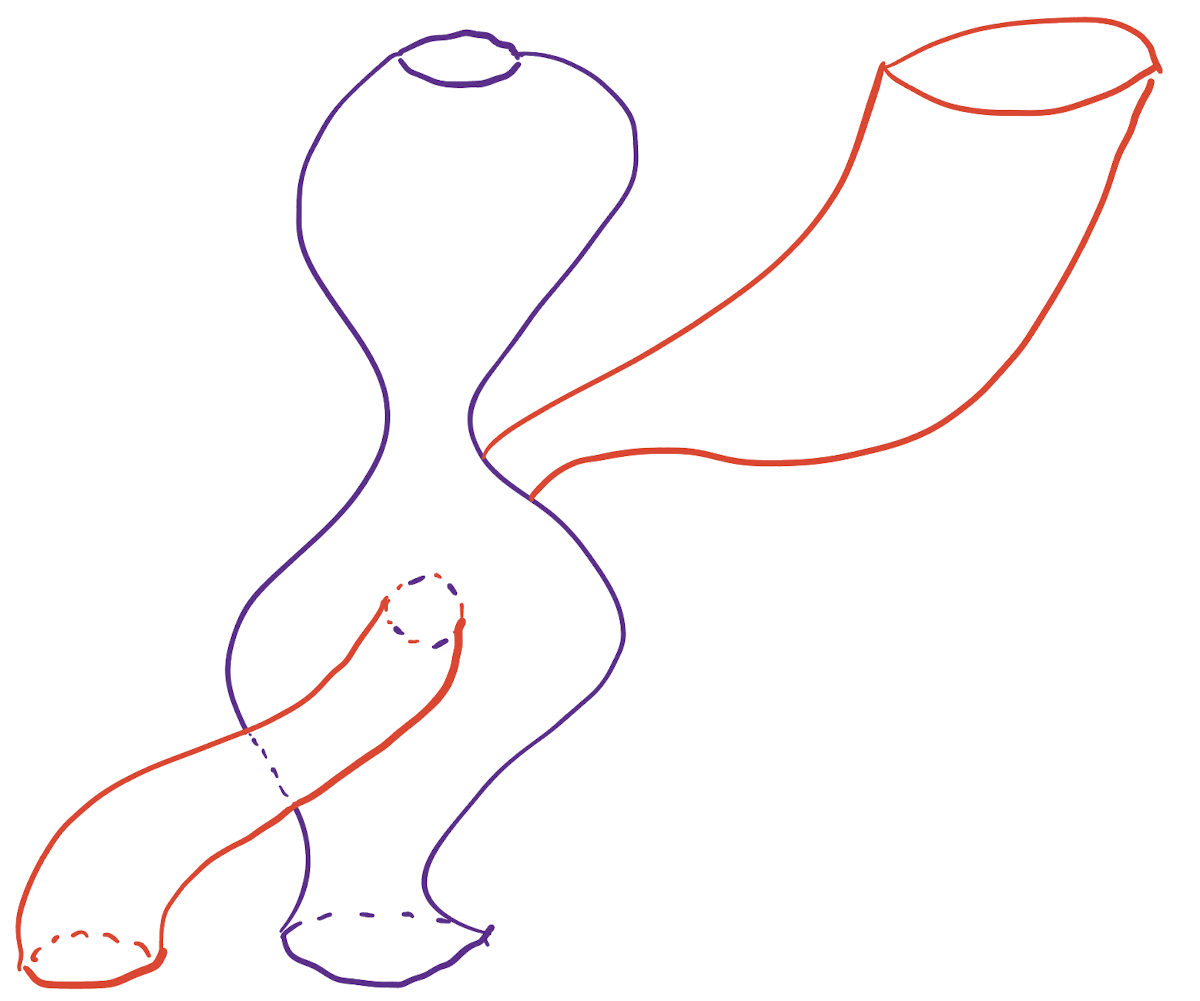
\includegraphics[scale = 0.18]{images/2D tubes on 2D plane as 3D shadow of 4D space.png}
    \end{center}
    % Place representative picture of braiding 2D tubes in 3D of the shadow of 4D space
    \begin{center}
    3D shadow of braid in 4D
    \end{center}
\end{frame}

\begin{frame}
    If we make our \( 4 \)th dimension time, then we have a movie of rings in \( 3 \)D. 
    % Image of the movie representation of 4D braids. 
    \begin{center}
        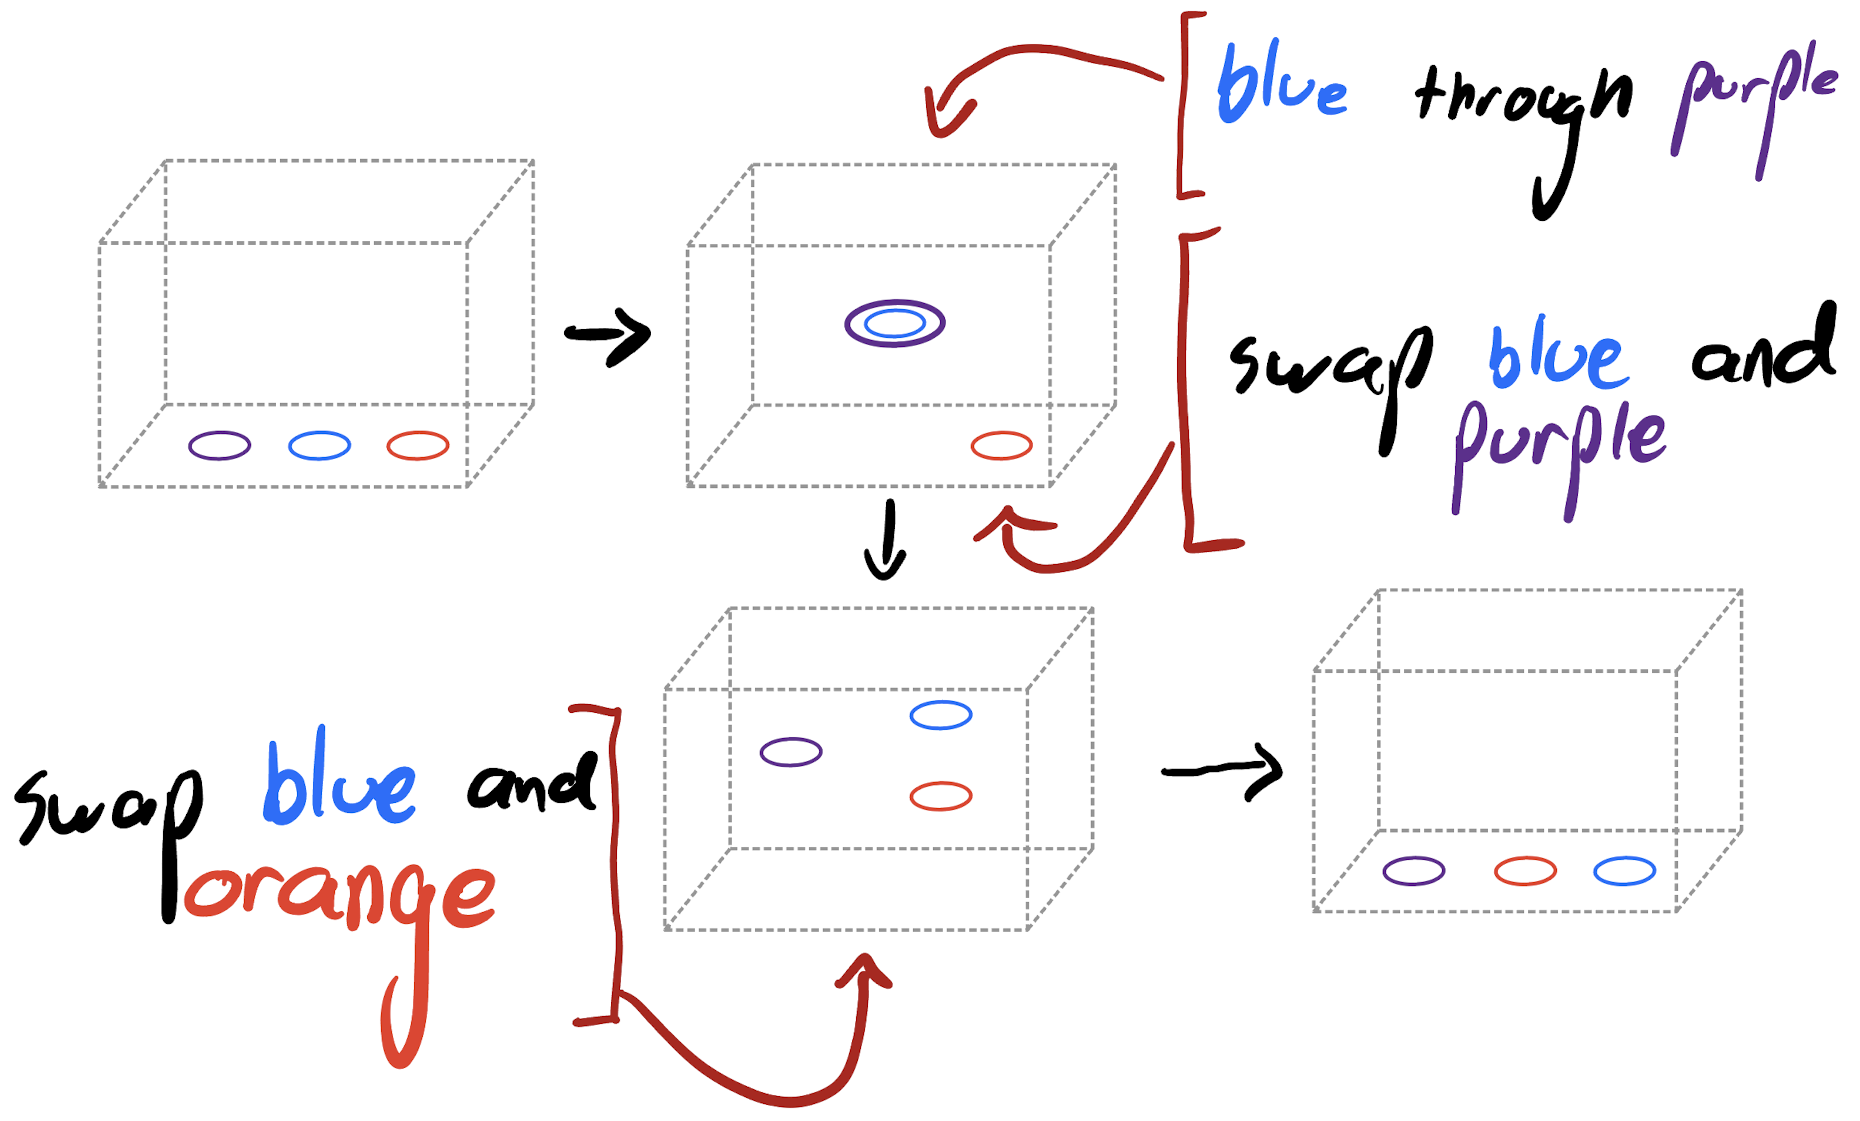
\includegraphics[width = \textwidth]{images/movie representation of a welded braid.png}
    \end{center}
\end{frame}

\begin{frame}
    \vfill
    \begin{tabular}{r l}
        ``Swap \( i \)th and \( (i + 1) \)th ring'' =& 
        \begin{minipage}{0.1\columnwidth}
        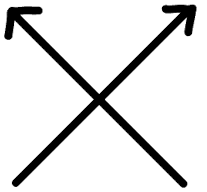
\includegraphics[scale = 0.17]{images/virtual crossing.png}
        \end{minipage} \\
    
        ``Cross \( i + 1 \)th ring through \( i \)th ring'' =&
        \begin{minipage}{0.1\columnwidth}
        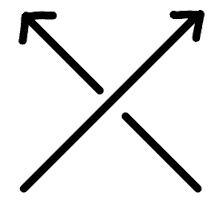
\includegraphics[scale = 0.17]{images/over crossing.png}
        \end{minipage} \\
    \end{tabular}
    
    \begin{center}
    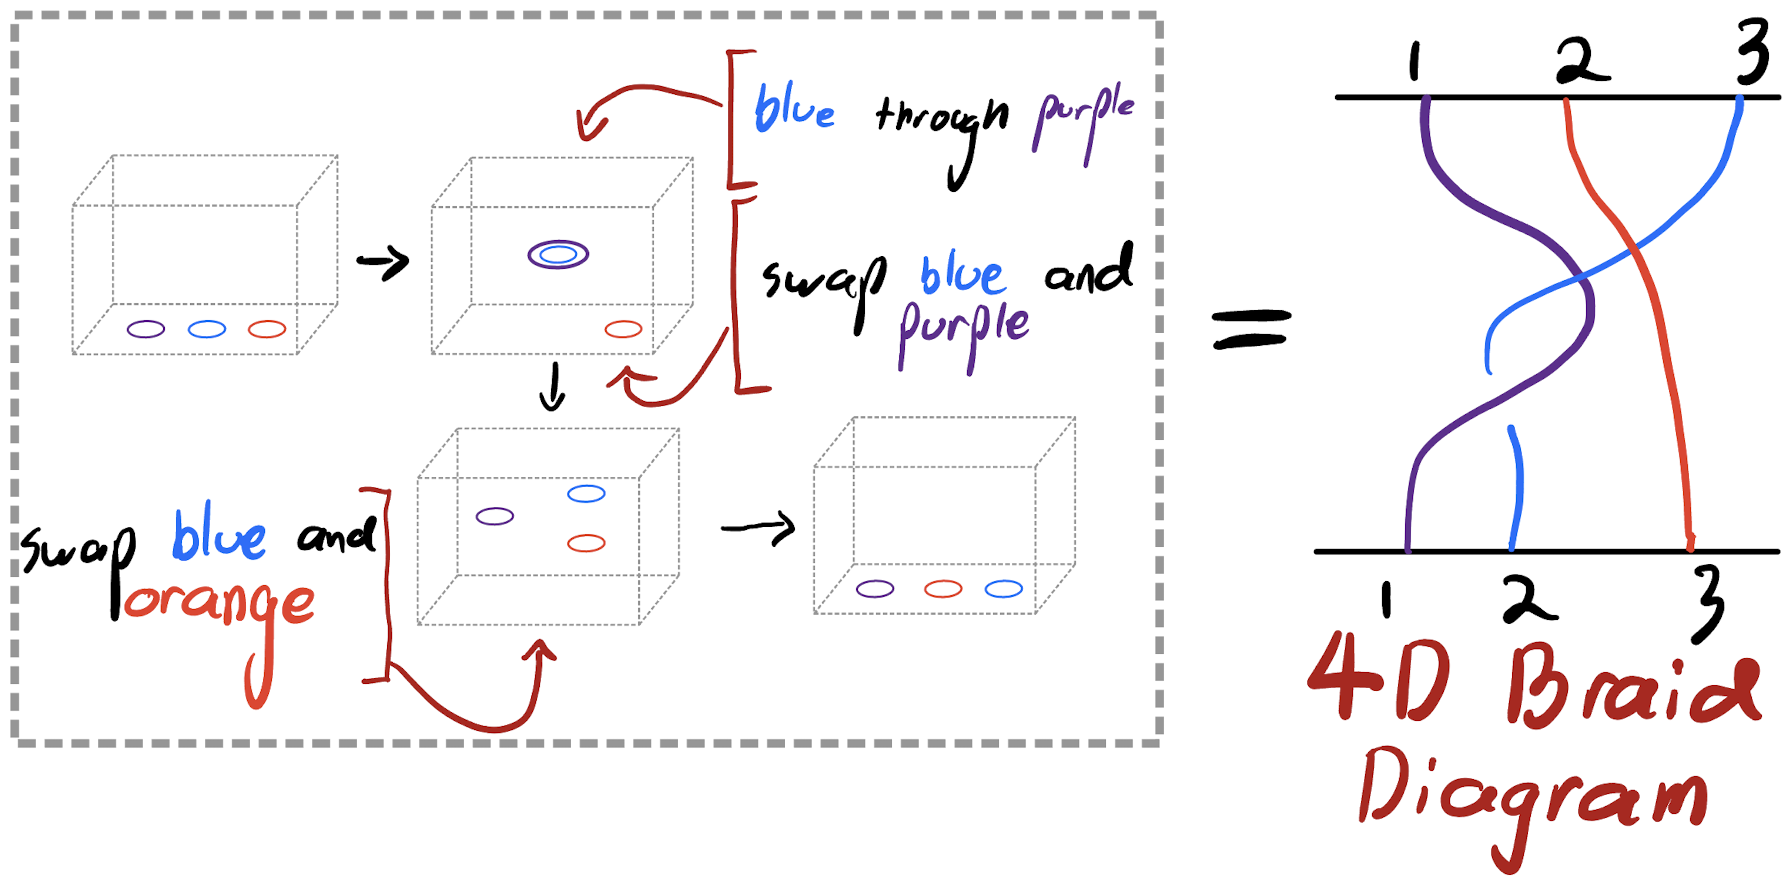
\includegraphics[width = \textwidth]{images/4D braid diagrams.png}
    \end{center}
    \vfill
    % Picture of movie to 4D braid diagram 
\end{frame}

\begin{frame}
    % Picture showing the equivalences between the flying rings, the 4D braid, and the 4D braid diagram. 
    \begin{center}
    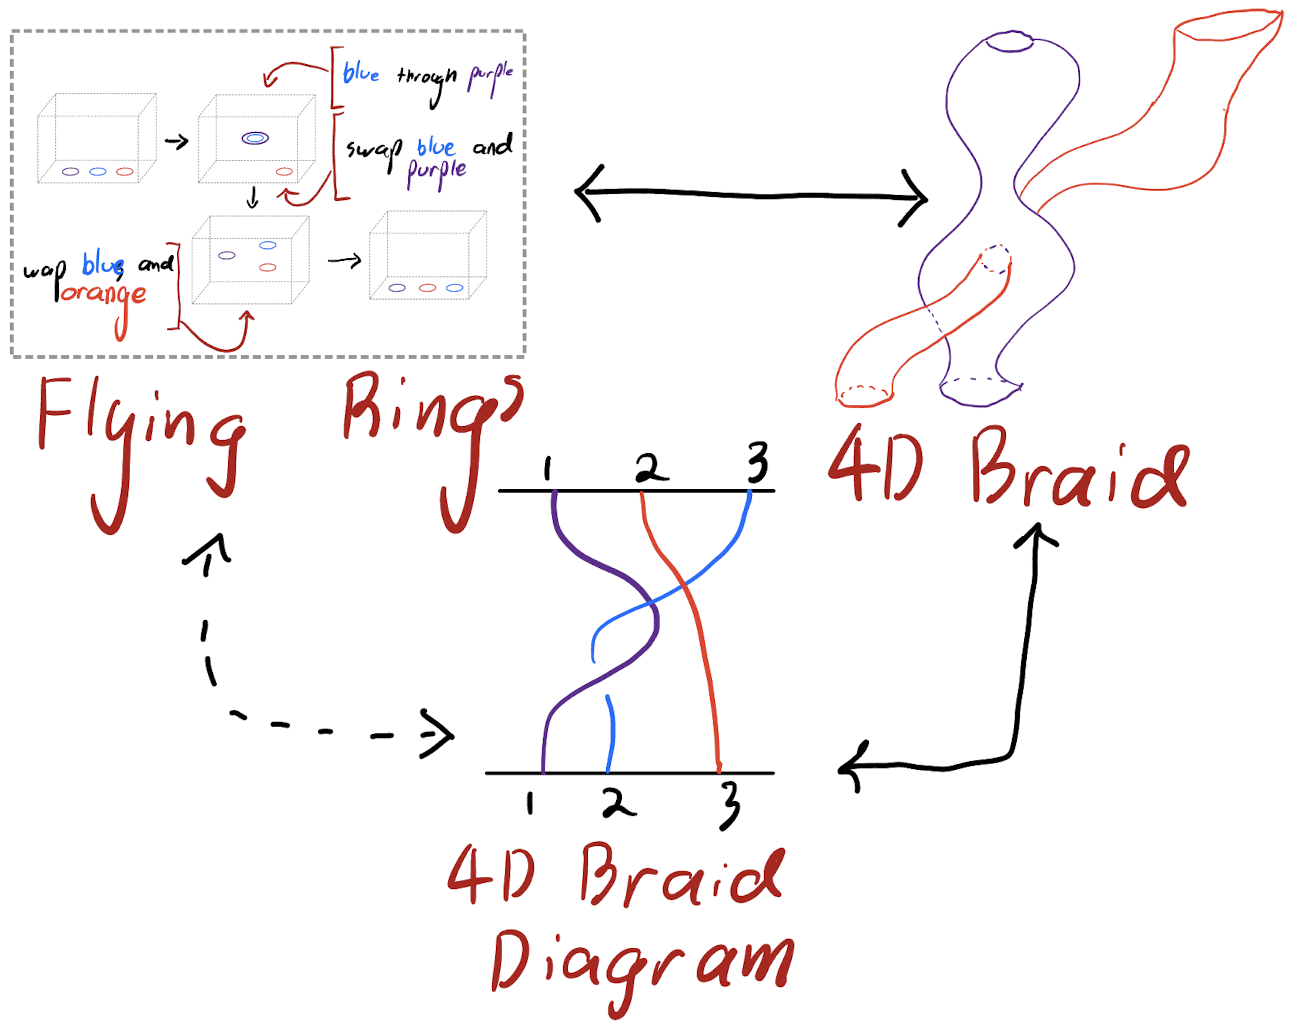
\includegraphics[width = \textwidth]{images/equivalences of welded braid representations.png}
    \end{center}
\end{frame}

\section{Do 4D Braids form a Canonical Operad Structure?}

\begin{frame}
    \begin{block}{Question}
        If we compose \Purple{4D Braids} like we do with \Purple{3D Braids}, does this form a \Purple{Canonical Operad Structure}?
    \end{block}
\end{frame}

\begin{frame}
    Let's test via example: 
    \vfill
    \begin{center}
    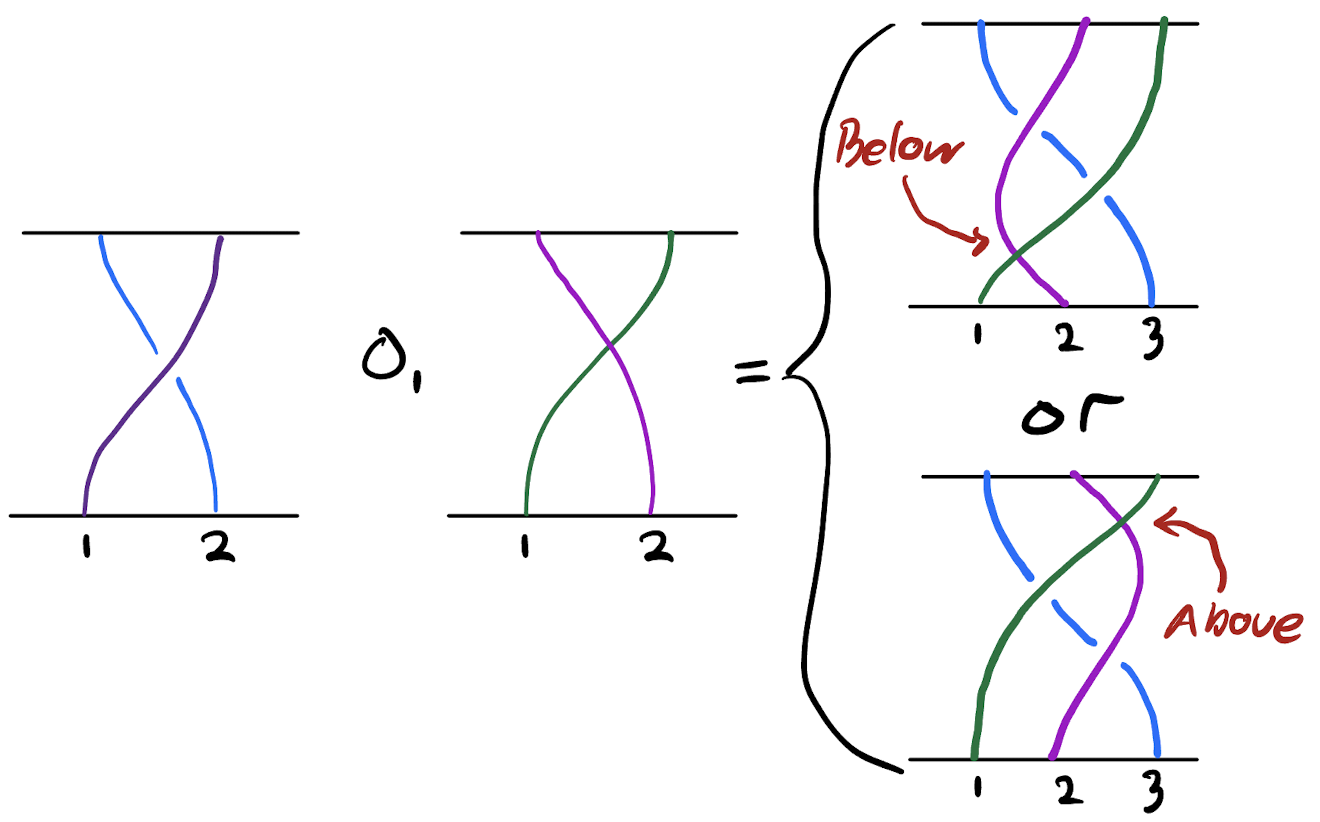
\includegraphics[width = \textwidth]{images/proof by picture.png}
    \end{center}
    For this operation to be well defined, we need the two 4D braid diagrams to describe the same braid. 
    
    % Picture of a 4D braid diagram being composed into a strand and getting two answers. 
\end{frame}
    
\begin{frame}
    \begin{center}
    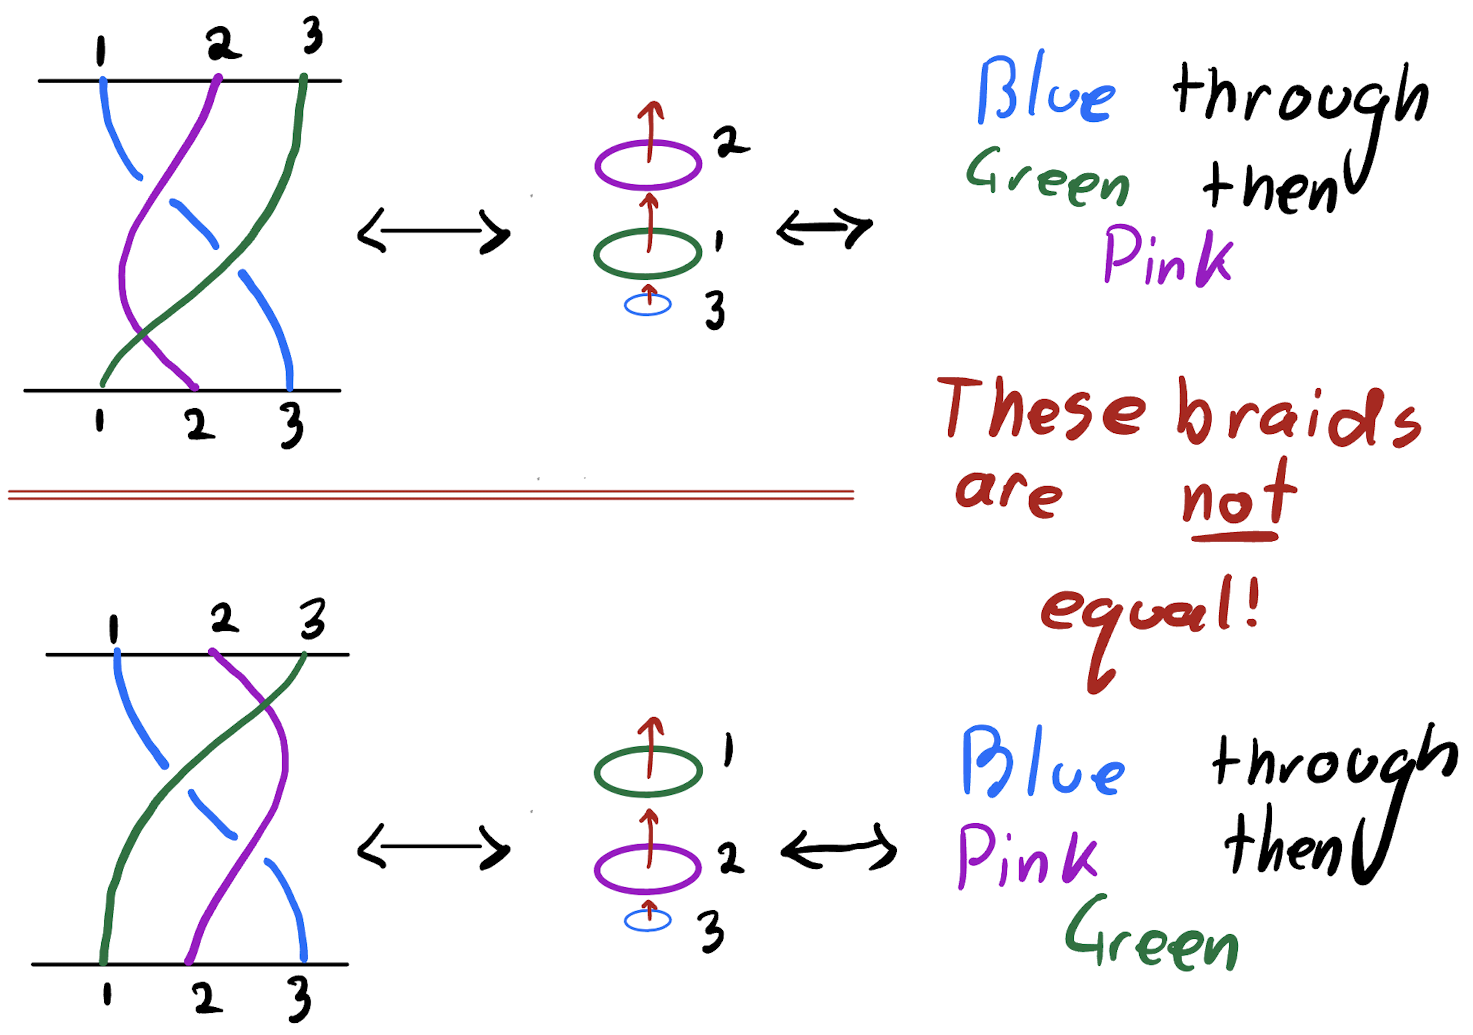
\includegraphics[width = \textwidth]{images/contradiction by picture.png}
    \end{center}
    % Showing that the two answers are fundamentally different using the ring intuition. 
\end{frame}

\begin{frame}
    With this contradiction it doesn't form an \Purple{Operad}...
    \pause
    However, if we make a convention that we always \\
    \begin{center}
        ``\Green{Do the crossings of the input braid first}'' \\
    \end{center}
    Then \Purple{4D Braids} form an \textcolor{Red}{non-canonical} \Purple{Operad}. 
\end{frame}

\begin{frame}
    \begin{block}{Answer}
        Yes, \( 4 \)D braids form an \Purple{Operad}. \\
        No, it is not \textcolor{Red}{Canonical}.
    \end{block}

    \begin{block}{Relevance}
        \Purple{ \( 3 \)D braids} forming an \Purple{Operad} is old news, however \Purple{\( 4 \)D braids} form an \Purple{Operad} is a new, previously unproved, result.
        This being said, this result is possibly unsurprising due to it's geometric intuition. 
    \end{block}

    \begin{theorem}
        4D Braids form a non-canonical operad under replacement of strands. 
    \end{theorem}
\end{frame}





\end{document}